\def\Lun{4}
\def\Ldeux{\Lun/3}
\def\Ltrois{\Ldeux/3}
Ex~: $l=27$
\begin{tikzpicture}[scale=0.9]
	\draw[black] (0,0) -- (0:\Lun) node[midway,above]{27};
\end{tikzpicture}
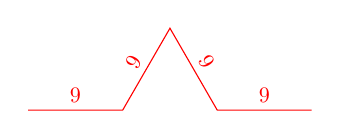
\begin{tikzpicture}[scale=0.9,every node/.style={scale=0.8}]
	\draw[red] (0,0)
			--++ (0:\Ldeux)
			node[midway,above,sloped]{9} --++ (60:\Ldeux)
			node[midway,above,sloped]{9} --++ (-60:\Ldeux)
			node[midway,above,sloped]{9} --++ (0:\Ldeux)
			node[midway,above,sloped]{9};
\end{tikzpicture}
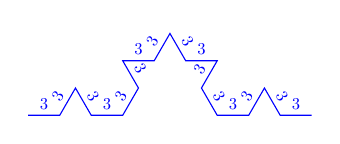
\begin{tikzpicture}[scale=0.9,every node/.style={scale=0.6}]
	\draw[blue] (0,0)
		--++ (0:\Ltrois)
		node[midway,above,sloped]{3} --++ (60:\Ltrois)
		node[midway,above,sloped]{3} --++ (-60:\Ltrois)
		node[midway,above,sloped]{3} --++ (0:\Ltrois)
		node[midway,above,sloped]{3} 
				
		--++ (60:\Ltrois)
		node[midway,above,sloped]{3} --++ (120:\Ltrois)
		node[midway,above,sloped]{3} --++ (0:\Ltrois)
		node[midway,above,sloped]{3} --++ (60:\Ltrois)
		node[midway,above,sloped]{3} 
				
		--++ (-60:\Ltrois)
		node[midway,above,sloped]{3} --++ (0:\Ltrois)
		node[midway,above,sloped]{3} --++ (-120:\Ltrois)
		node[midway,above,sloped]{3} --++ (-60:\Ltrois)
		node[midway,above,sloped]{3} 
				
		--++ (0:\Ltrois)
		node[midway,above,sloped]{3} --++ (60:\Ltrois)
		node[midway,above,sloped]{3} --++ (-60:\Ltrois)
		node[midway,above,sloped]{3} --++ (0:\Ltrois)
		node[midway,above,sloped]{3};
\end{tikzpicture}